\documentclass[conference]{IEEEtran}
\usepackage{iftex}
% IEEE style uses Times: TeX Gyre Termes under XeTeX/tectonic, newtx under pdfLaTeX.
\ifXeTeX
  \usepackage{fontspec}
  \setmainfont{texgyretermes}[Extension=.otf, UprightFont=*-regular, BoldFont=*-bold, ItalicFont=*-italic, BoldItalicFont=*-bolditalic]
\else
  \usepackage[T1]{fontenc}
  \usepackage{newtxtext,newtxmath}
\fi
\usepackage{cite}
\usepackage{amsmath}
\usepackage{graphicx}
\usepackage[hidelinks]{hyperref}

\begin{document}

\title{Masking Neural Network Cores for Security}

\author{\IEEEauthorblockN{Ajay Sabareesh Balamurugan and Kaiyuan Yang}
\IEEEauthorblockA{Department of Electrical and Computer Engineering\\
Rice University, Houston, TX, USA\\
ELEC594 Capstone --- Midterm Report, Fall 2026}}

\maketitle

\begin{abstract}
Edge AI accelerators leak their weights through power consumption, and masking---splitting every
secret into random shares---is the principled defense, but it is costly. Where that cost lands depends on the
masking domain. Boolean shares make logic cheap and addition expensive, while arithmetic shares do the opposite,
so hybrid designs convert between the two. We follow that cost across four masked designs for a digital
in-memory compute (DIMC) accelerator evaluated on VGG16. Each redesign moved the cost to a different block---the adder
tree, weight storage, fresh randomness, and finally the Boolean-to-arithmetic conversion---rather than removing
it. In the current design, one masked product of an 8-bit weight takes 16 logic gates to compute but 150 to
convert into arithmetic shares, so making the converter smaller is our next objective. We also brought up
HDCIM, a 28\,nm hybrid-protected DIMC chip from our lab, on a test bench, and leakage measurements
follow next.
\end{abstract}

\section{Introduction}
Neural networks deployed on edge accelerators carry trained weights that are valuable intellectual property,
and the hardware running them sits physically in an adversary's hands. Side-channel measurements have been shown
to reveal a network's architecture and parameters~\cite{batina2019csinn}, and in-memory computing (IMC)
architectures, whose weights stay stationary inside the array, are particularly exposed~\cite{wang2024imc}.

Masking is the principled defense. Every secret value is split into random shares, so that no single wire
carries it. Its price, however, is high. Published masked accelerators pay heavily for that protection~\cite{maji2023ti},
and a masked digital IMC macro gives up $6.2\times$ in area efficiency~\cite{ashok2025imc}. That cost is not spread evenly, because which operations
become expensive depends on how the secret is split, as the next section explains. Our objective is affordable masking
for digital in-memory compute (DIMC)~\cite{chih2021dimc}, and the first step is to understand where its cost comes from.

This report makes three contributions. First, it traces where the masking cost lands across four successive
masked designs of a DIMC accelerator. Second, it quantifies the cost of the Boolean-to-arithmetic conversion that
dominates the current design, at the level of a single product. Third, it reports the post-silicon bring-up of
HDCIM~\cite{pakala2024thesis}, a taped-out hybrid-protected DIMC chip, as the platform for measuring leakage on
real silicon.

\section{Methods}\label{sec:methods}
\subsection{Masking Domains}
Masking splits each secret $x$ into random shares, and the number of shares depends on the security order. A
circuit secure against an attacker who probes $d$ wires needs at least $d+1$ shares~\cite{ishai2003private}. This
work targets first-order security, where any single probed wire must be independent of $x$, so the minimum is two
shares. There are two ways to split it. In the Boolean domain $x = x_1 \oplus x_2$, and XOR acts on each share
separately,
\begin{equation}
x \oplus y = (x_1 \oplus y_1) \oplus (x_2 \oplus y_2).
\end{equation}
A product, however, expands into four terms,
\begin{equation}
x \cdot y = x_1 y_1 \oplus x_1 y_2 \oplus x_2 y_1 \oplus x_2 y_2 ,
\end{equation}
and the two cross terms combine shares, so they must be re-randomized with fresh random bits and held in
registers to stay secure~\cite{gross2016dom}. Every carry of an adder is such a product, which makes addition
expensive in the Boolean domain. In the arithmetic domain $x = x_1 + x_2 \bmod 2^n$, and addition becomes
share-wise and cheap. Any operation that needs the bits of $x$, such as the sign test inside ReLU, now depends
on the carries between both shares, and arithmetic shares must also be stored at the full width of the
accumulator.

A neural network needs both cheap logic and cheap addition. Fully Boolean designs pay in their adder
trees~\cite{ashok2025imc}, arithmetic designs pay in their nonlinear layers~\cite{dubey2020maskednet}, and
hybrid designs keep each domain where it is cheap and convert between them~\cite{dubey2022modulonet}. The
Boolean-to-arithmetic (B2A) conversion~\cite{goubin2001b2a,shahmirzadi2024b2a} is itself nonlinear, so it
brings a cost of its own.

\subsection{Design Progression and Cost Accounting}
We model the datapath of a DIMC accelerator in five stages, namely weight storage, in-array multiply, adder
tree, accumulation, and batch normalization with ReLU, with a conversion inserted wherever a design changes
domain. Four designs were evaluated in sequence, each chosen to remove the bottleneck of the one before. The
first, an earlier approach, used an XNOR multiply with a three-share Boolean carry-save adder tree, whose
adder was synthesized in TSMC 28\,nm and assessed by fixed-versus-random test vector leakage assessment (TVLA)
on simulated power traces, where a Welch $t$-statistic beyond $\pm 4.5$ flags first-order
leakage~\cite{schneider2015tvla}. The later three use two shares, target first-order security under the glitch-extended probing model
gadget by gadget, and are costed over VGG16 on CIFAR-10 with 8-bit weights and activations.

Costs are counted per block in separate units, namely two-input logic gates, adder cells, storage bits, fresh
random bits, registers and latency. They are never summed, because a design that saves registers while adding gates has
made a trade rather than a saving. Each design is compared with its own unprotected counterpart. Network-level
compute figures weight each layer by its share of multiply-accumulate operations, and storage is totalled over the
whole network. As a check on this counting, applying it to the published B2A converter~\cite{shahmirzadi2024b2a}
at 32-bit width gives 126 registers, exactly the number its authors report.

\subsection{HDCIM Test Bench}
HDCIM~\cite{pakala2024thesis} is an earlier masked DIMC design from our lab, fabricated in TSMC 28\,nm. It places a masked DIMC
core next to an unmasked twin of the same core on separate supplies, which gives a built-in leaky reference. The
masked core multiplies with a secure Boolean AND~\cite{kumar2023glitchy} and, instead of masking the B2A
conversion, places it on its own supply behind a switched-capacitor current equalizer that flattens its power
signature. Every register on the chip is reached through a single 5,148-bit scan chain.

Fig.~\ref{fig:bench} shows the bench we built around it. A PC drives the scan chain through an NI PCIe-6536B
digital I/O card and an isolator on the chip board, an NI PCIe-6738 analog output card supplies a tunable delay
rail, and an oscilloscope monitors the on-chip clocks.

\begin{figure}[t]
\centering
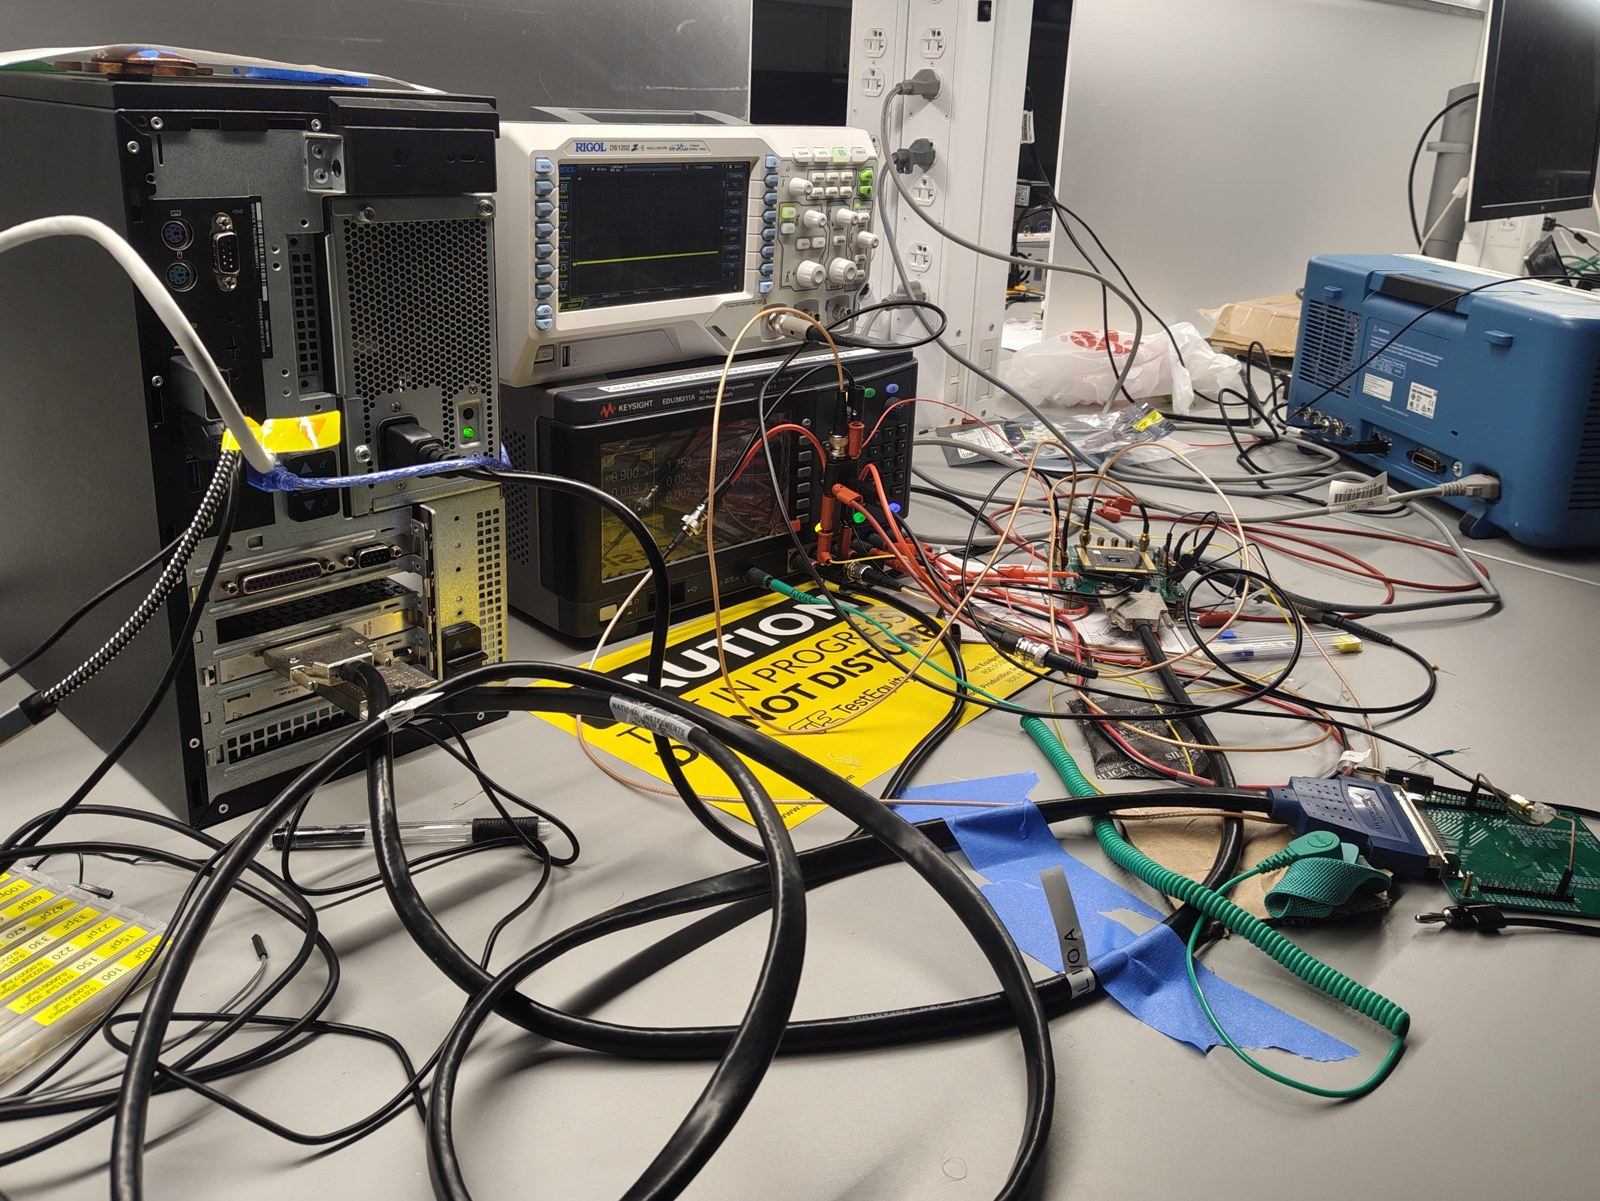
\includegraphics[width=\columnwidth]{figures/bench.jpg}
\caption{HDCIM test bench. A PC with NI digital I/O and analog output cards drives the chip board through its
scan chain, and an oscilloscope monitors the on-chip clocks.}
\label{fig:bench}
\end{figure}

\section{Results (Partial)}
\subsection{Where the Cost Landed}
Fig.~\ref{fig:journey} traces the four designs through the same datapath, with the block that carried most of
the masking cost shown in red. In the first design the cost sat in the adder tree. In simulated TVLA its unmasked
adder reached a $t$-statistic of about 20. Fig.~\ref{fig:tvla} shows the three-share version staying within
$\pm 4.5$ over 60,000 traces, while a cheaper hybrid with only two shares in the carry chain peaked near $t=-10$
and therefore leaked, which closed that route to a smaller tree.

The second design used arithmetic shares throughout, so every addition became share-wise. The shares, however,
had to be stored at accumulator width and the multiply produced four product lanes, so across VGG16 weight
storage grew $7.19\times$ and adder cells $11.08\times$ over the unprotected design, at $3.5\times$ its latency.
The third design kept the weights in Boolean shares, multiplied them with a masked AND and converted each product
to arithmetic shares. Storage fell back to $2.00\times$, but every masked AND needs fresh randomness, and the
masked multiply alone drew about 5,550 random bits per cycle. The fourth and current design replaces the AND with an
XNOR, which is linear over Boolean shares and needs no fresh randomness. Storage stays at $2.00\times$ and adder
cells fall to $7.59\times$ at $3.44\times$ latency. Each step lowered the cost it targeted and raised another, so
the masking cost moved rather than shrank. Table~\ref{tab:cost} lists these costs side by side in their separate
units. Its random-bit rows show the XNOR removing the multiply's fresh randomness while the converter's demand
stays about the same.

\begin{figure}[t]
\centering
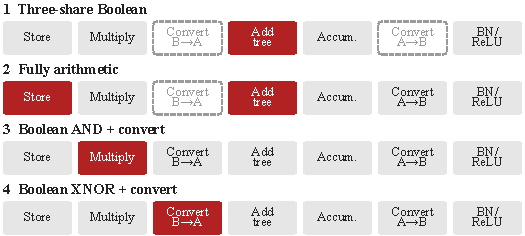
\includegraphics[width=\columnwidth]{figures/journey.pdf}
\caption{Where the masking cost landed in each of the four designs. Red marks the dominant block, and dashed
boxes mark stages the design does not have.}
\label{fig:journey}
\end{figure}

\begin{table}[t]
\centering
\caption{Cost of Designs 2--4 in Separate Units}
\label{tab:cost}
\footnotesize
\setlength{\tabcolsep}{4pt}
\begin{tabular}{lccc}
\hline
 & 2 Fully & 3 Boolean & 4 Boolean \\
 & arithmetic & AND + convert & XNOR + convert \\
\hline
Weight storage & $7.19\times$ & $2.00\times$ & $2.00\times$ \\
Adder cells & $11.08\times$ & $7.32\times$ & $7.59\times$ \\
Random bits/cycle & & & \\
\quad in multiply & 0 & 5,554 & 0 \\
\quad in conversion & 5 & 21,317 & 22,086 \\
Latency & $3.5\times$ & $3.44\times$ & $3.44\times$ \\
Converter bank $N$ & 1 & 768 & 768 \\
\hline
\end{tabular}

\vspace{3pt}
\parbox{\columnwidth}{\scriptsize Ratios are against each design's own unprotected counterpart for VGG16 on
CIFAR-10 with 8-bit weights and activations. Logic and latency are weighted by multiply-accumulate operations and
storage is totalled over the whole network. Random bits are absolute, weighted the same way, and assume no sharing
of randomness between gadgets.}
\end{table}

\subsection{One Product, Computed and Converted}
Fig.~\ref{fig:product} isolates a single product in the current design. Computing it takes 16 two-input gates,
one XNOR per bit of the 8-bit weight in each of the two shares. Converting it into 26-bit arithmetic shares takes
150 gates, nearly ten times as many. The converter also holds 85 registers and draws 26 fresh random bits per
conversion, which are counted separately and are first-order, gadget-level figures that do not imply composable
security. Every product passes through a conversion, so the converter rather than the multiply now sets the
cost of the masked datapath, and making it smaller is the main objective for the rest of the project.

\begin{figure}[t]
\centering
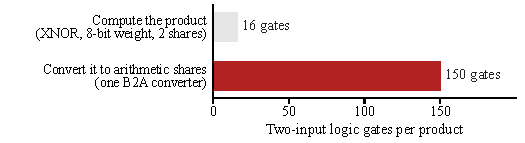
\includegraphics[width=\columnwidth]{figures/product.pdf}
\caption{Two-input gates needed for one masked product in the current design, to compute it and to convert it
into arithmetic shares.}
\label{fig:product}
\end{figure}

\begin{figure}[t]
\centering
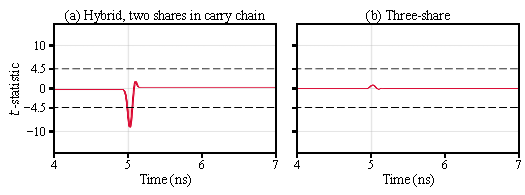
\includegraphics[width=\columnwidth]{figures/tvla.pdf}
\caption{Simulated fixed-versus-random TVLA of the first design's adder over 60,000 traces, with dashed lines at
the $\pm 4.5$ threshold. (a) Hybrid with two shares in the carry chain. (b) Three-share adder.}
\label{fig:tvla}
\end{figure}

\subsection{HDCIM Bring-Up}
The bench now operates the chip end to end, and Table~\ref{tab:bringup} lists each check. The one fault found
was in the memory, where the first overnight run returned wrong reads until the clock was stopped before each
address change. Power traces have not yet been taken.

\begin{table}[t]
\centering
\caption{HDCIM Bring-Up Checks}
\label{tab:bringup}
\footnotesize
\begin{tabular}{ll}
\hline
Check & Result \\
\hline
Scan chain & 5,148 of 5,148 bits \\
On-chip clocks & Run in both modes \\
Memory read-back, unmasked & 0 bad reads in 976 \\
First overnight memory run & 328 of 852 wrong \\
\quad clock stopped before address change & 0 wrong \\
Unmasked compute, near-memory MAC & Verified \\
Masked mode & Characterised \\
\hline
\end{tabular}
\end{table}

\section{Discussion (Partial)}
The progression shows that redesigning a masked datapath moves its cost rather than removing it, and in the
current design that cost sits in the B2A converter. Two lines of work follow toward the final presentation of this project. The first
verifies every masked block with SILVER and PROLEAD, searches for a smaller converter, and compares converting
once per product against once per neuron. The second adds a power-sense tap to the HDCIM board and runs TVLA on
the masked core against its unmasked twin. Three limitations apply. The design costs are counted gates rather
than synthesized area, the effect of the XNOR weight grid on network accuracy has not been measured, and the
silicon results will come from one chip at room temperature.

\section*{Acknowledgments}
The authors thank the Secure and Intelligent Micro-Systems (SIMS) Lab and the Department of Electrical and
Computer Engineering at Rice University for their support, and Akhil Reddy Pakala for the design of the HDCIM
chip.

\section*{CRediT Author Statement}
\noindent\textbf{Ajay Sabareesh Balamurugan:} Conceptualization, Methodology, Software, Validation, Formal Analysis,
Investigation, Visualization, Writing -- Original Draft, Writing -- Review \& Editing.

\noindent\textbf{Kaiyuan Yang:} Supervision, Writing -- Review \& Editing.

\bibliographystyle{IEEEtran}
\bibliography{refs}

\end{document}
